\documentclass[tikz,border=10pt]{standalone}
\usepackage{amsmath}
\usepackage{tikz}
\usetikzlibrary{arrows.meta, positioning, calc, shapes.geometric}

\begin{document}
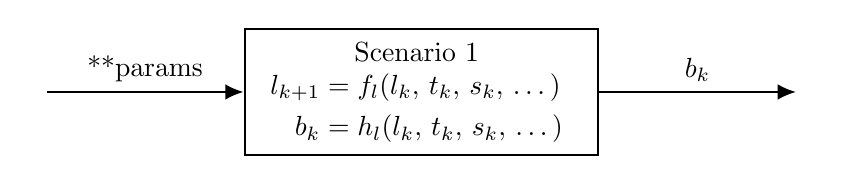
\begin{tikzpicture}[
  block/.style = {draw, thick, minimum height=3em, minimum width=6em, align=center},
  arrow/.style = {thick, -{Latex[width=2mm]}},
  node distance=2.5cm and 2.5cm
]

  \node[block] (button) {
    \begin{tabular}{c}
      Scenario 1 \\
      $\begin{aligned}
        l_{k+1} &= f_l(l_k,\,t_k,\,s_k,\,\dots) \\
        b_k &= h_l(l_k,\,t_k,\,s_k,\,\dots)
      \end{aligned}$
    \end{tabular}
  };

  % params input from the left
  \node[left=2.5cm of button] (params) {};
  \draw[arrow] (params.east) -- node[above] {**params} (button.west);

  % b_k output to the right
  \node[right=2.5cm of button] (bout) {};
  \draw[arrow] (button.east) -- node[above] {$b_k$} (bout.west);

\end{tikzpicture}
\end{document}
